\documentclass[12pt,a4j,twocolumn]{jarticle}

\usepackage{graphicx}

\title{LaTeXの使い方}
\author{1821013  岩谷 慶}
\date{\today}

%%%%%%%%%%%%%%%%%%%%
%\renewcommand\baselinestretch{0.8}
%\renewcommand\figurename{Fig.}
%%%%%%%%%%%%%%%%%%%%

\begin{document}

\maketitle

%%%%%%%%%%%%%%%%%%%%
%\pagestyle{empty}
%\thispagestyle{empty}
%%%%%%%%%%%%%%%%%%%%

%%%%%%%%%%%%%%%%%%%%
\section{数式のラベル参照}\label{sec_label}
第\ref{sec_label}節では、以下の連立微分方程式から2階微分方程式を導出する。
%
\begin{eqnarray}
  \label{eq:x}
  xxx & = & yyy \\
	\label{eq:dx}
	\frac{dx}{dt} & = & y \\
	\label{eq:dy}
	\frac{dy}{dt} & = & - x - 2 \delta y 
\end{eqnarray}
%
式(\ref{eq:dx})を式(\ref{eq:dy})に代入すると、
式(\ref{eq:ddx})が導出される。
%
\begin{equation}
	\label{eq:ddx}
	\frac{d^2x}{dt^2} + 2 \delta \frac{dx}{dt} + x = 0
\end{equation}

\newpage

%%%%%%%%%%%%%%%%%%%%
\section{figure環境}

関数$y=\sin(x)$のグラフを図\ref{fg:sin}に示し、
関数$y=\cos(x)$のグラフを図\ref{fg:cos}に示す。
%
%\begin{figure}[b]
\begin{figure}[tb]
	\begin{center}
	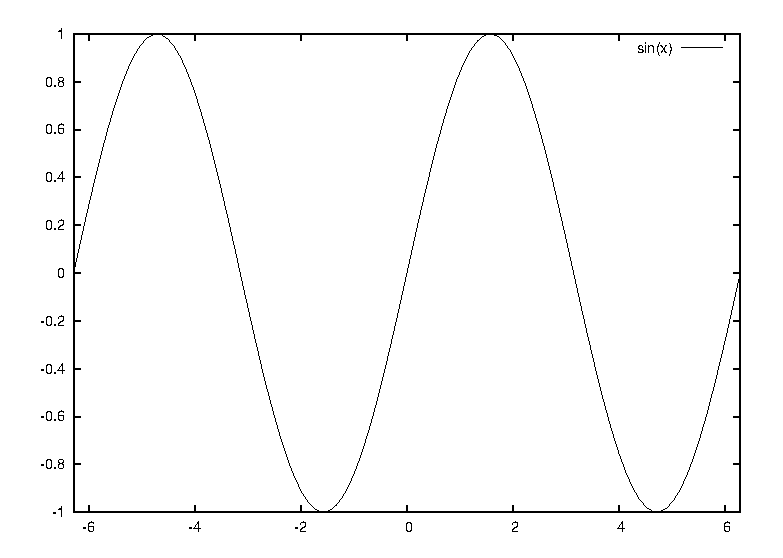
\includegraphics[width=6cm]{sin.eps}
	\end{center}
	%%%%%%%%%%%%%%
	%\vspace*{-5mm}
	%%%%%%%%%%%%%%
	\caption{sin関数}
	\label{fg:sin}
\end{figure}
%
\begin{figure}[tb]
	\begin{center}
	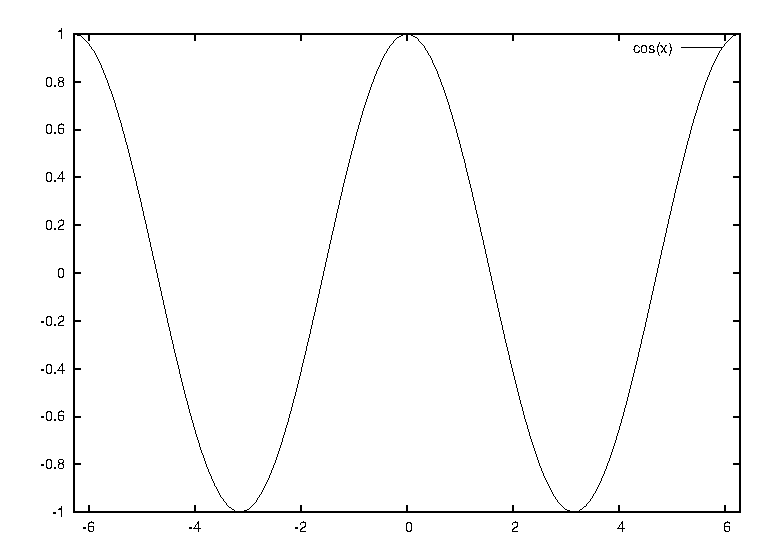
\includegraphics[width=6cm]{cos.eps}
	\end{center}
	%%%%%%%%%%%%%%
	%\vspace*{-5mm}
	%%%%%%%%%%%%%%
	\caption{cos関数}
	\label{fg:cos}
\end{figure}

%%%%%%%%%%%%%%%%%%%%
%\pagestyle{plain}
%\setcounter{page}{5}
%%%%%%%%%%%%%%%%%%%%

\newpage

%%%%%%%%%%%%%%%%%%%%
\section{table環境}

OR関数$y = x_1 + x_2$の真理値表を表\ref{tb:or}に示し、
AND関数$y = x_1 \cdot x_2$の真理値表を表\ref{tb:and}に示す。

\begin{table}[tb]
	\caption{OR関数の真理値表}
	\label{tb:or}
	\begin{center}
	  \begin{tabular}{|c|c||c|}
		\hline
		$x_1$ & $x_2$ & $y$ \\ \hline\hline
		    0 &     0 &   0 \\ \hline
		    0 &     1 &   1 \\ \hline
		    1 &     0 &   1 \\ \hline
		    1 &     1 &   1 \\ \hline
	\end{tabular}
	\end{center}
\end{table}

\begin{table}[tb]
	\caption{AND関数の真理値表}
	\label{tb:and}
	\begin{center}
	\begin{tabular}{|c|c||c|}
		\hline
		$x_1$ & $x_2$ & $y$ \\ \hline \hline
		    0 &     0 &   0 \\ \hline
		    0 &     1 &   0 \\ \hline
		    1 &     0 &   0 \\ \hline
		    1 &     1 &   1 \\ \hline
	\end{tabular}
	\end{center}
\end{table}

\newpage

%%%%%%%%%%%%%%%%%%%%
\section{thebibliography環境}

TeXに関するコマンドをもっと詳しく調べたい場合は、\cite{tex1}-\cite{tex6}などの参考書を入手しましょう!
特に、文献\cite{tex2,tex5}は重要です!

\begin{thebibliography}{9}
\bibitem{tex1} 奥村晴彦, LaTeX2e美文書作成入門, 技術論社
\bibitem{tex2} 中野賢, 日本語LaTeX2eブック, アスキー
\bibitem{tex3} 海上忍, 黒川弘章, これだけでできるLaTeX実践活用ガイド, 技術論社
\bibitem{tex4} 乙部厳己, 江口庄英, pLaTeX2e for Windows, ソフトバンクパブリッシング
\bibitem{tex5} 土屋勝, 誰でもできるやさしいTeX入門, カットシステム
\bibitem{tex6} 藤田眞作, LaTeX2eコマンドブック, ソフトバンク
\end{thebibliography}

\end{document}
